\documentclass{beamer}

\usepackage[utf8]{inputenc}
\usepackage{minted}
\usepackage{listings}
\usepackage{graphicx}
\usepackage{xcolor}
%\usepackage{adjustbox}
\usepackage{adjustbox}


%\usetheme{metropolis}
%\usecolortheme{beaver}
\usetheme{Madrid}
\useinnertheme{circles}
\definecolor{ssgreen}{HTML}{669B41}
\usecolortheme[named=ssgreen]{structure}
\setbeamertemplate{navigation symbols}{}

\AtBeginEnvironment{frame}{\setcounter{footnote}{0}}

\title[Kubernetes]{Introduction to Kubernetes}
\author[Ed MacDonald]{Ed MacDonald\\emacdonald@solutionstreet.com}
\institute[\href{https://solutionstreet.com}{SolutionStreet}]{SolutionStreet\\\href{https://solutionstreet.com}{(solutionstreet.com)}}
\date{July 2020}

\begin{document}
\frame{\titlepage}

\begin{frame}
\frametitle{What is Kubernetes?}
A Container Orchestration Framework
\end{frame}

\begin{frame}
\frametitle{Kubernetes API}
The Kubernetes API is how you interact with Kubernetes. Most Kubernetes API calls involve either:
\begin{itemize}
    \item You telling Kubernetes what you want the state of a given set of objects to converge to, or
    \item You asking Kubernetes what the current state of a given set of objects is
\end{itemize}
\end{frame}

\begin{frame}
\frametitle{Kubernetes API}
Think of the Kubernetes API as a way to:
\begin{itemize}
    \item Send YAML documents to Kubernetes specifying components you would like to create.
    \item Send requests to Kubernetes to update components.
    \item Send requests asking Kubernetes for the current state of components.
\end{itemize}
\end{frame}

\begin{frame}
    \begin{center}
        \Huge Tools
    \end{center}
\end{frame}

\begin{frame}
    \frametitle{minikube\footnotemark}
    \begin{itemize}
        \item Easiest way to install a cluster on your machine.
        \item For development purposes only!
    \end{itemize}
    \footnotetext[1]{https://kubernetes.io/docs/tasks/tools/install-minikube}
\end{frame}

\begin{frame}
    \frametitle{docker client\footnotemark}
    \begin{itemize}
        \item We need to be able to build and publish our images to minikube's docker server.
    \end{itemize}
    \footnotetext[1]{https://www.docker.com/get-started}
\end{frame}

\begin{frame}
\frametitle{kubectl\footnotemark}
\begin{itemize}
\item Used to communicate with Kubernetes clusters.
\item Provides a convenient way to speak with Kubernetes via its API.
\item We'll be using it to update components in our cluster and view their state.
\item You \textbf{\textit{can}} use it to create components, but there is a better way to do that...
\end{itemize}
\footnotetext[1]{https://kubernetes.io/docs/tasks/tools/install-kubectl}
\end{frame}

\begin{frame}
\frametitle{helm\footnotemark}
\begin{itemize}
    \item Tool for packaging and deploying Kubernetes apps.
    \item Think of as a way to package and deploy all the YAML files that specify components in your app.
\end{itemize}
\footnotetext[1]{\href{https://helm.sh}{https://helm.sh}}
\end{frame}

\begin{frame}
    \begin{center}
        \Huge Kubernetes Architecture Overview With Sample Apps
    \end{center}
\end{frame}

\begin{frame}
\frametitle{Kubernetes Nodes}
\begin{itemize}
\item The compute instances (virtual machines, bare metal servers) running the Kubernetes software components that make up a Kubernetes cluster.
\item Kubernetes schedules Pods (which make up your Applications) to run on these nodes.
\end{itemize}
\end{frame}

% https://www.patrickbaylis.com/posts/2018-10-11-beamer-resizing/
\begin{frame}
    \frametitle{Kubernetes Nodes}
    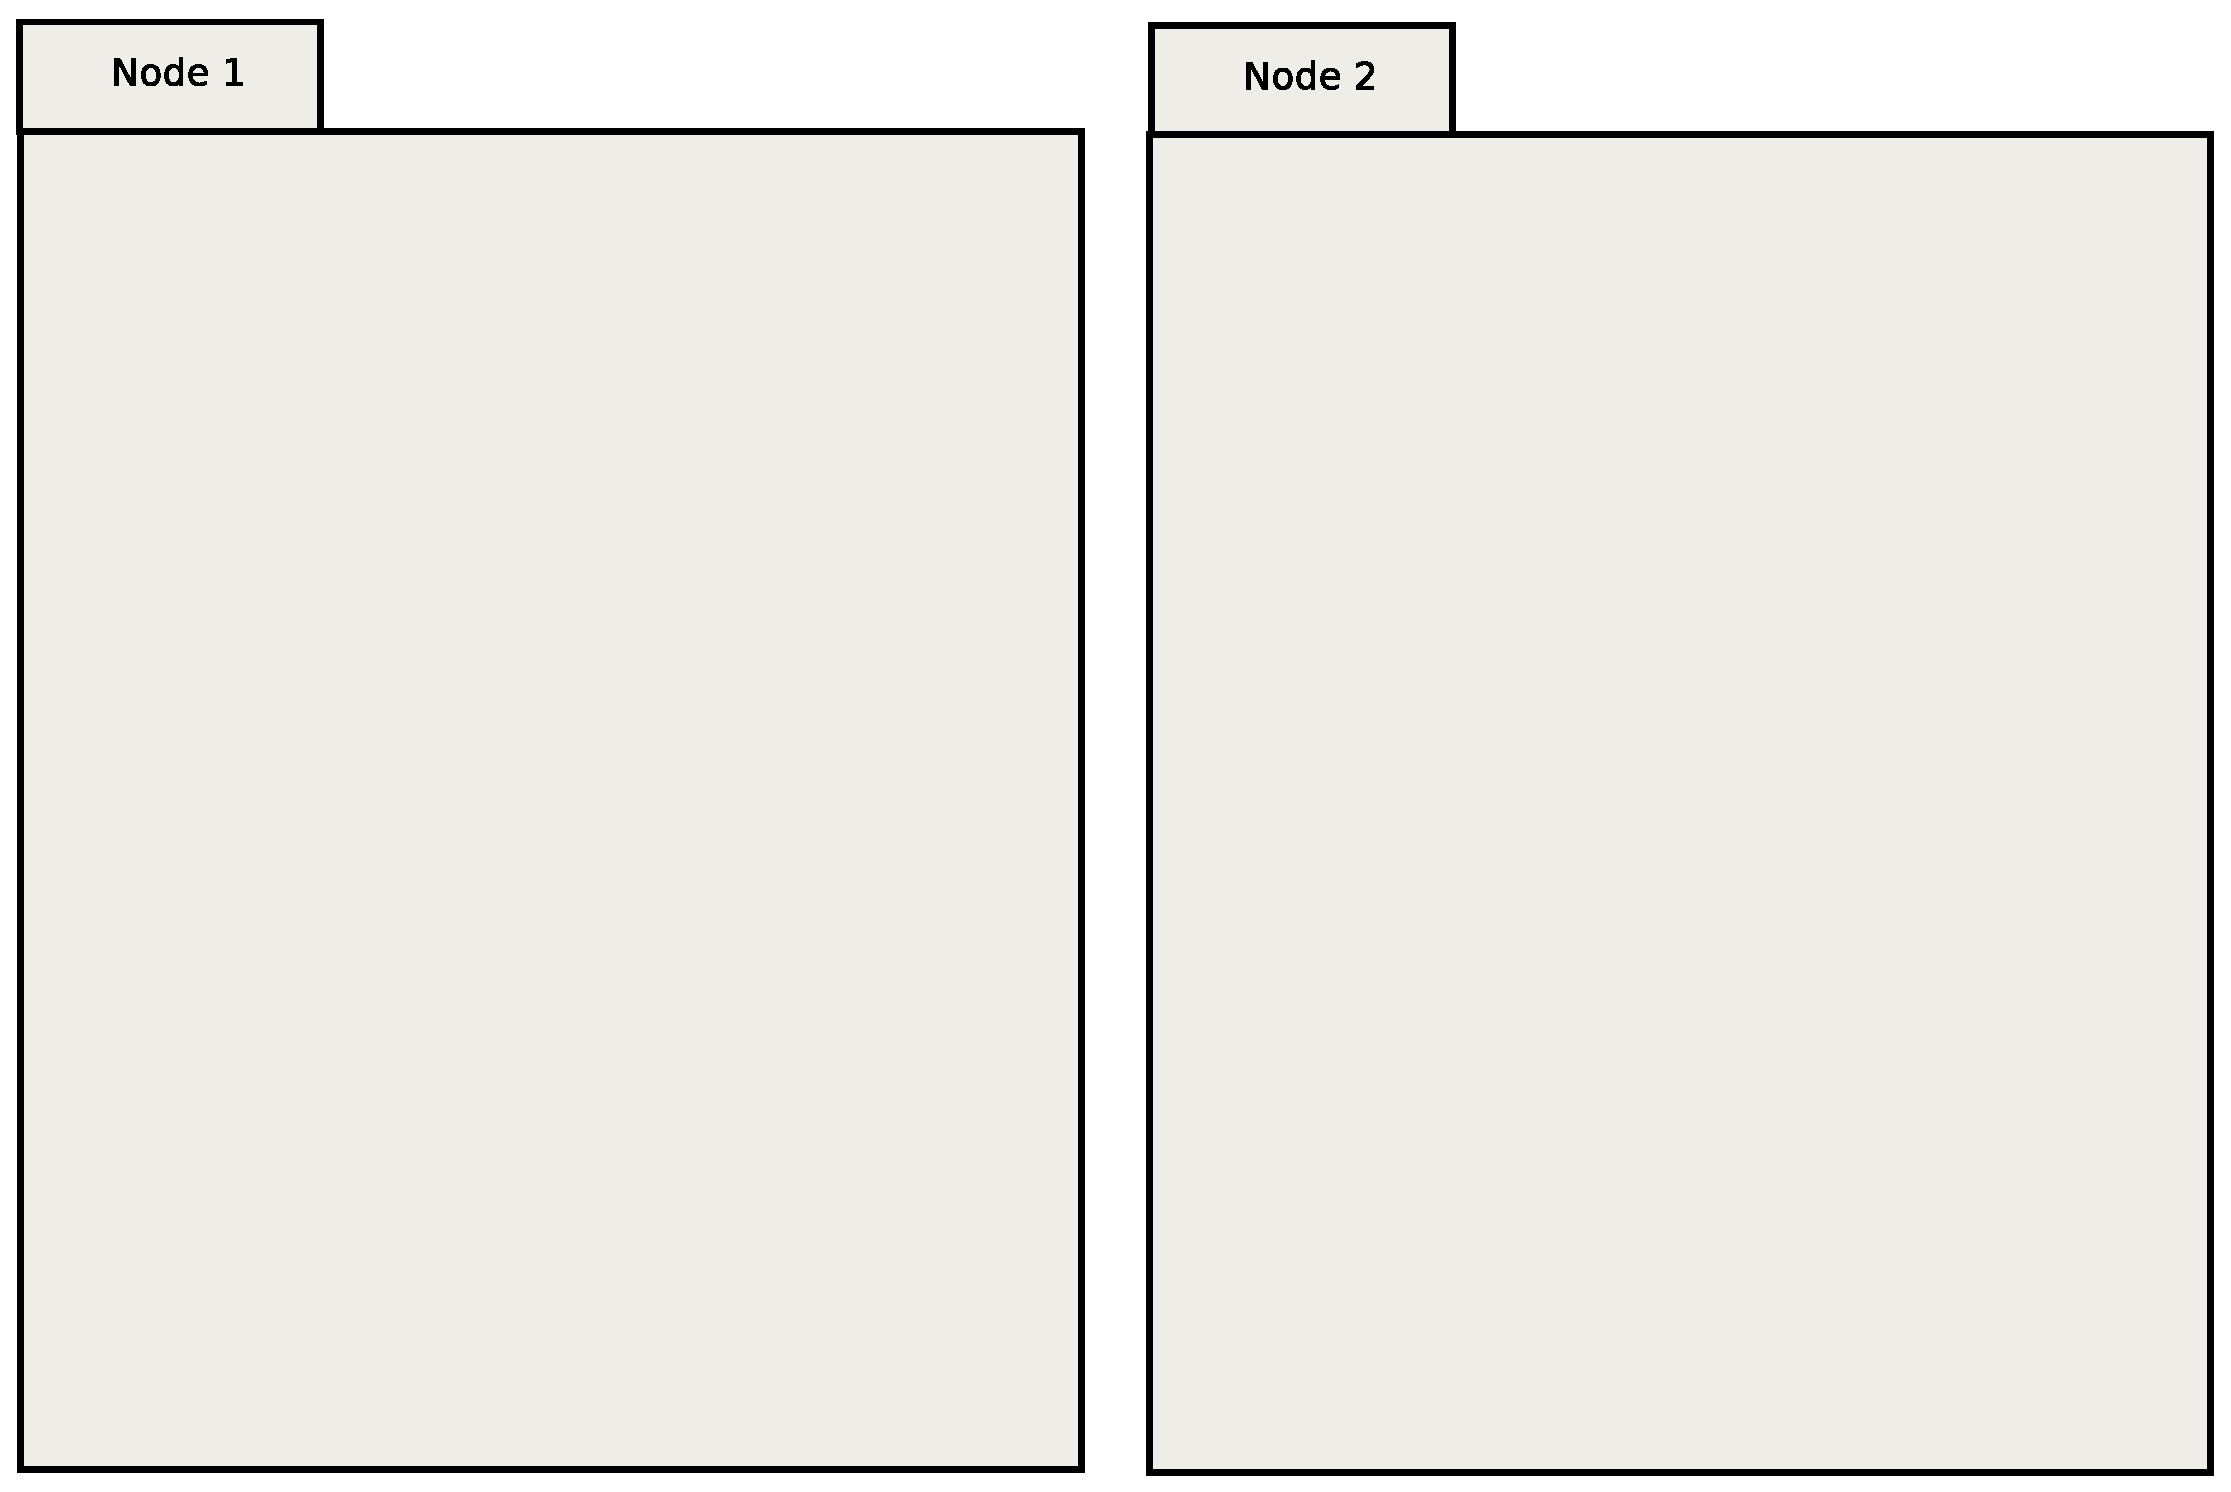
\includegraphics[width=\textwidth,height=0.85\textheight,keepaspectratio]{graphics/00-nodes.eps}
\end{frame}

\begin{frame}
\frametitle{Pods}
Pods (not containers!) are the fundamental building blocks of a Kubernetes application
\begin{itemize}
    \item A Pod is a group of one or more containers that work closely together on a specific task.
    \item Containers in a Pod can access the same volumes.
    \item Some Containers in a Pod can be Init Containers, which run before other pods start and are used to perform initialization tasks.
\end{itemize}
\end{frame}

\begin{frame}
    \frametitle{System Pods}
    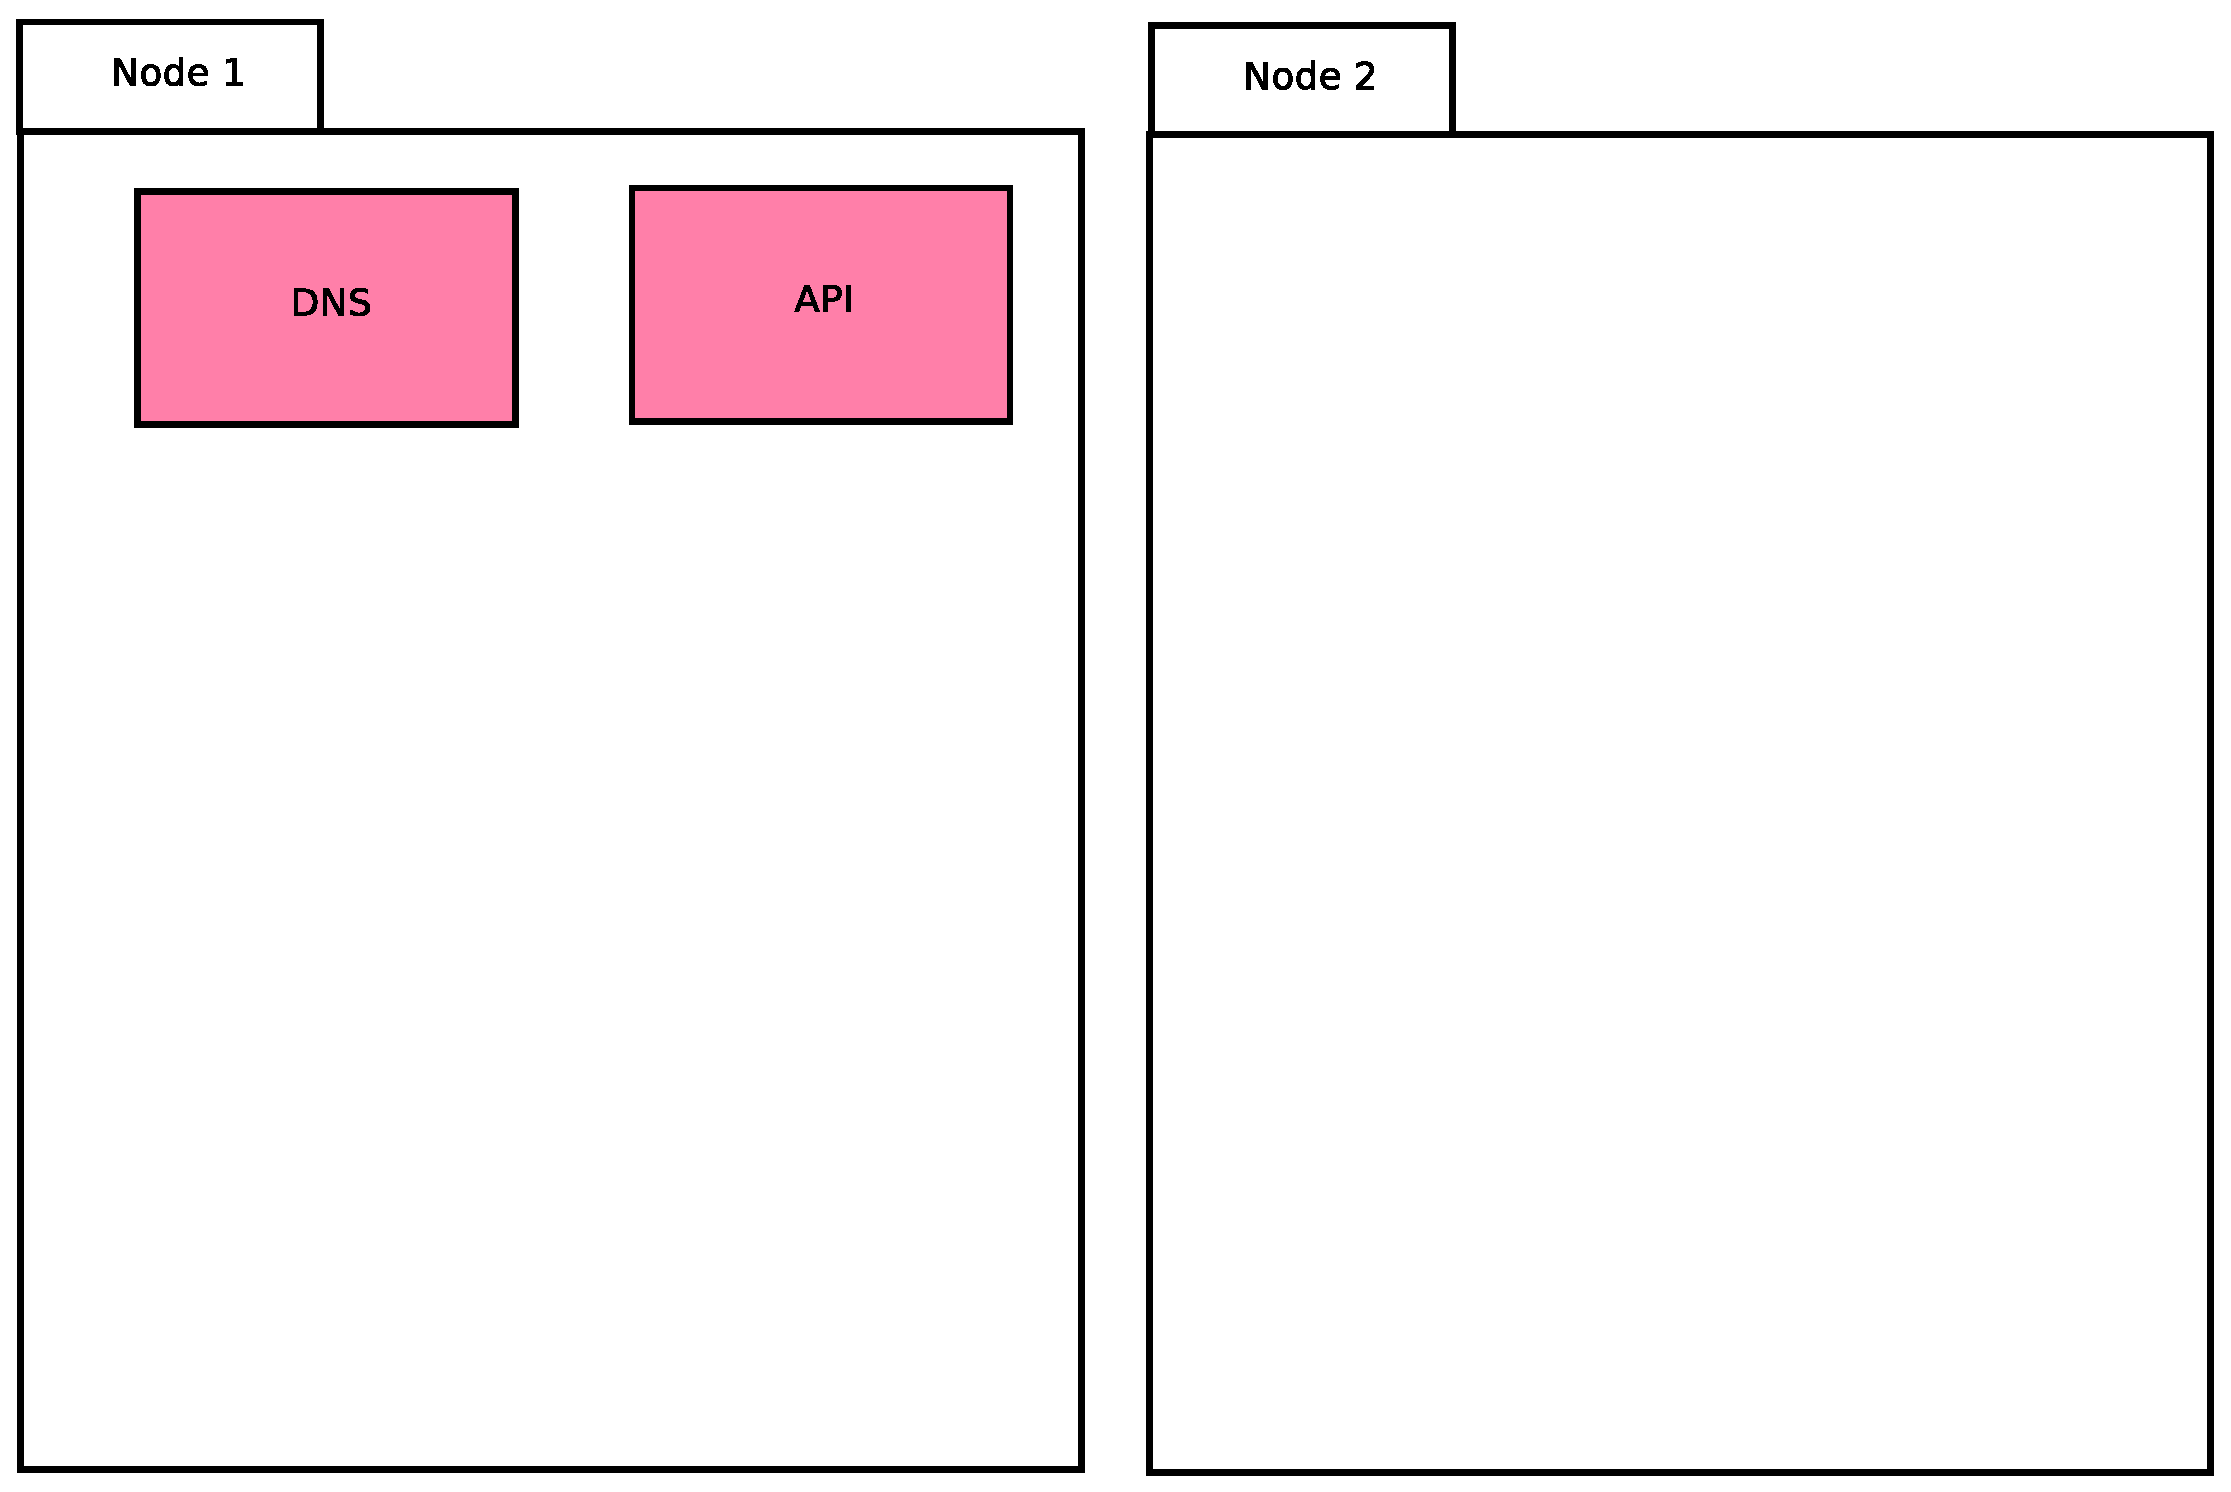
\includegraphics[width=\textwidth,height=0.85\textheight,keepaspectratio]{graphics/01-systemPods.eps}
\end{frame}

\begin{frame}
\frametitle{The Sample Apps}
I wrote two apps that do nothing other than suggest a random Subreddit.
\begin{itemize}
    \item One is stateless and selects at random from a list of 280 Subreddits.
    \item The other is stateful and removes each Subreddit from the list upon suggesting it.
\end{itemize}
\end{frame}

\begin{frame}
    \frametitle{Stateless Application Pods}
    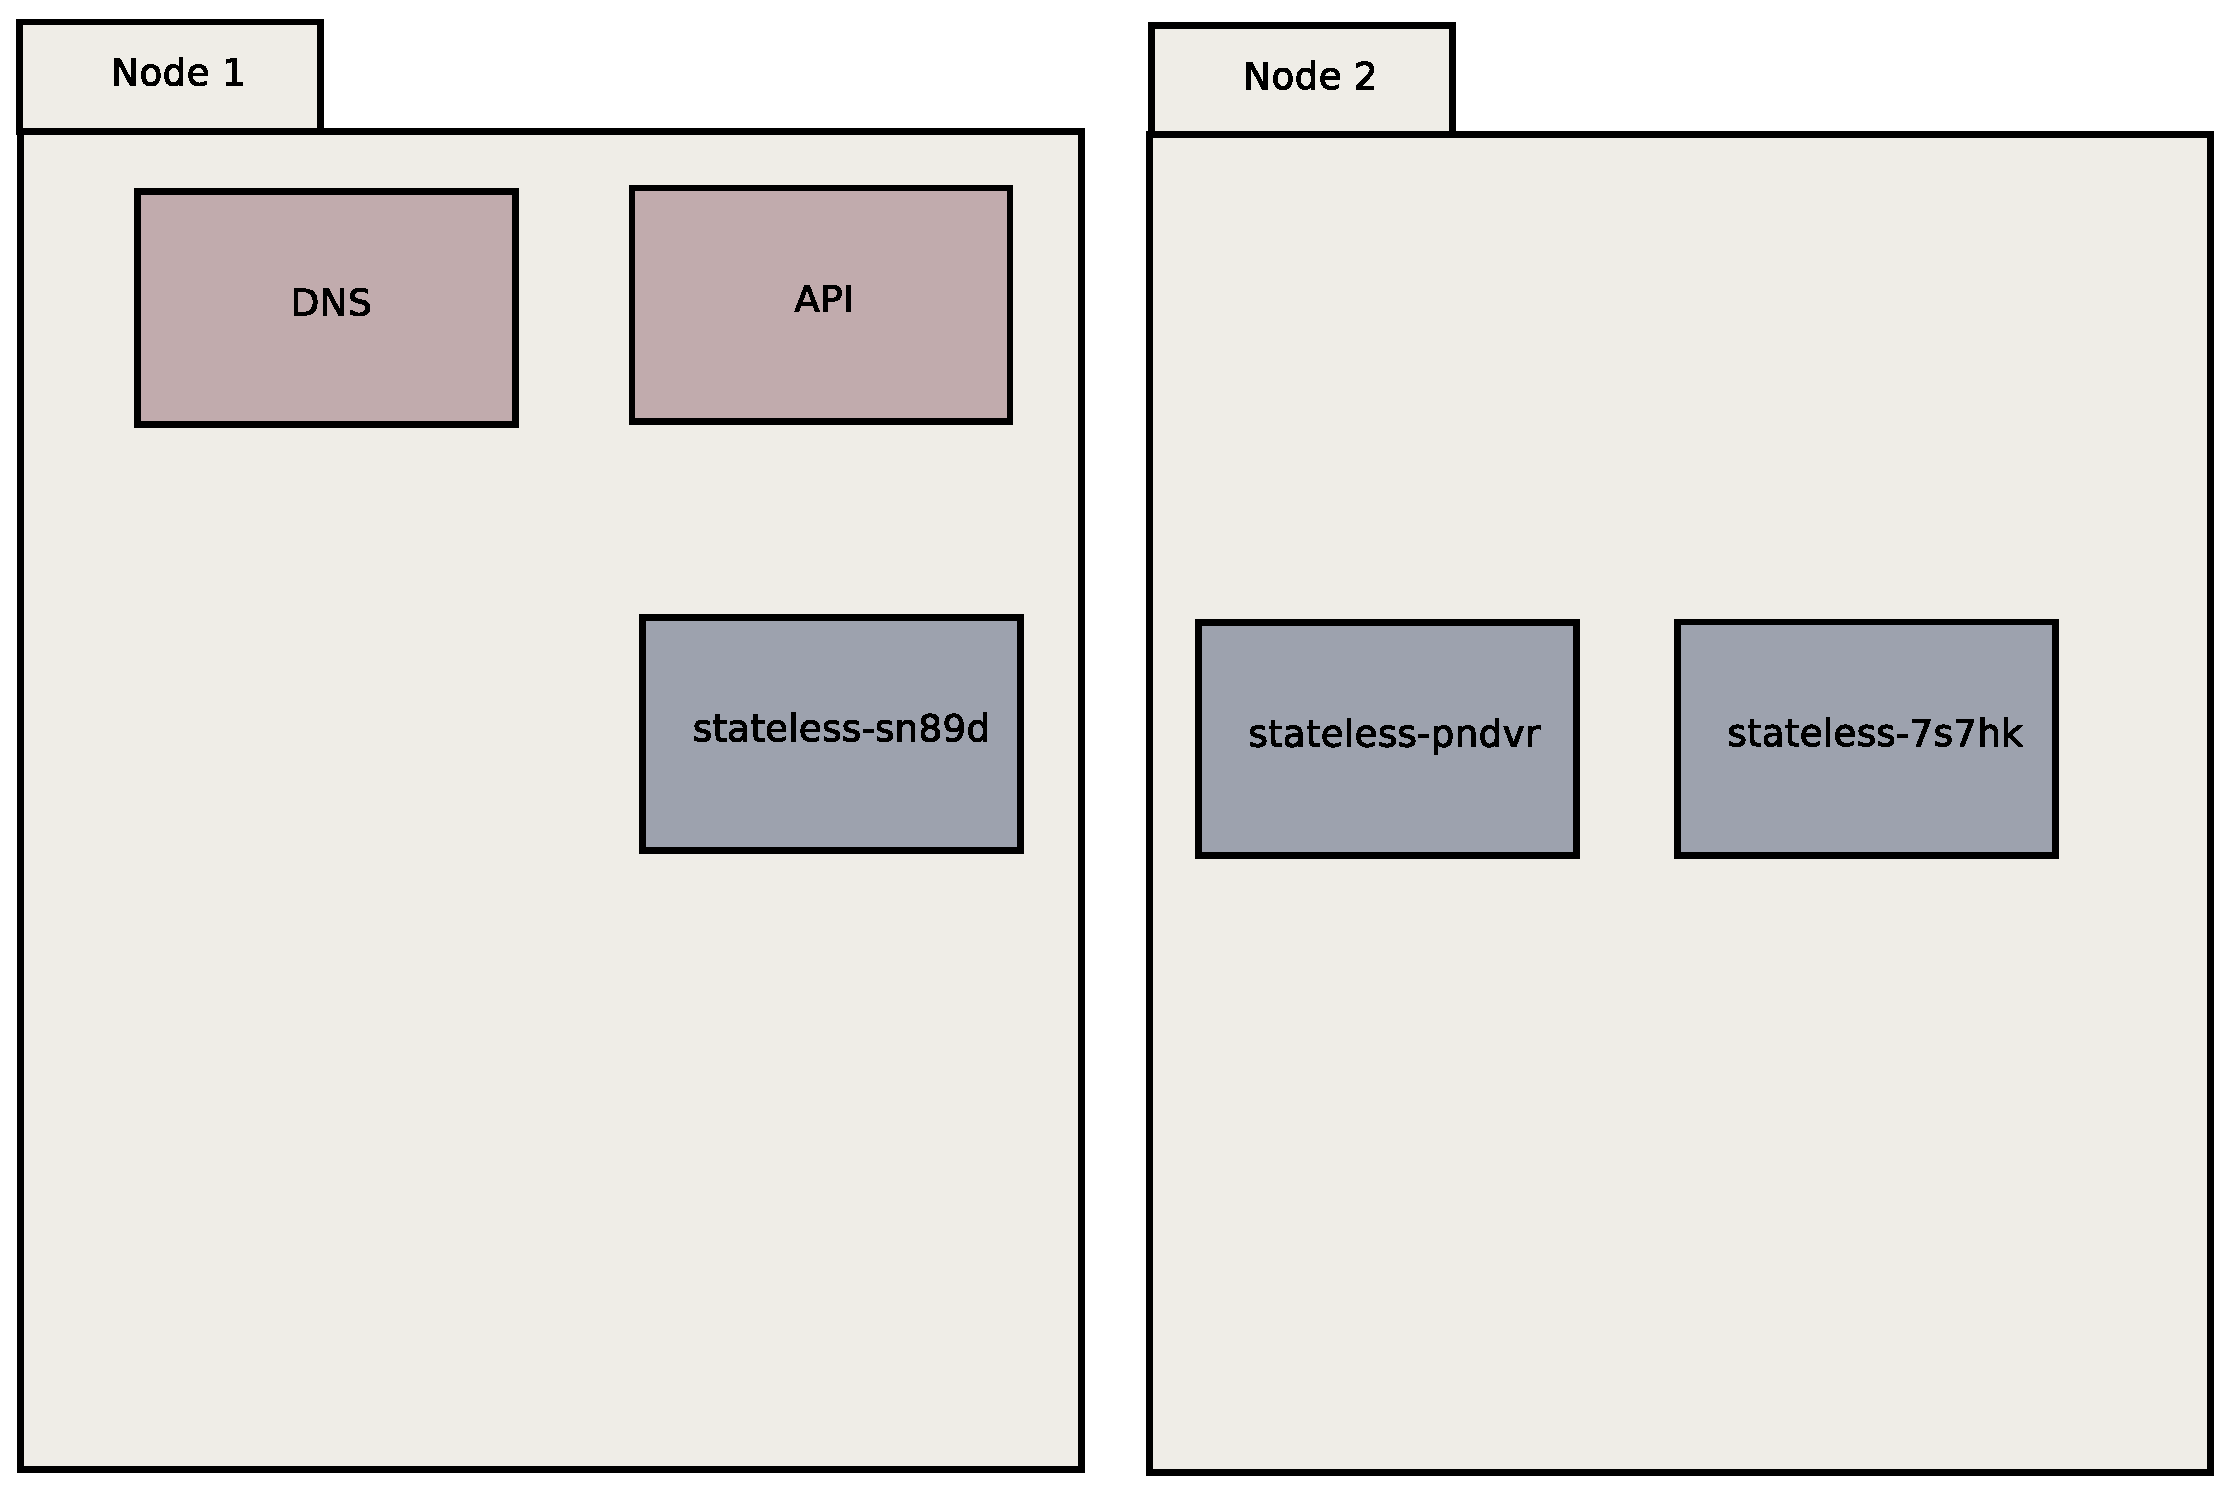
\includegraphics[width=\textwidth,height=0.85\textheight,keepaspectratio]{graphics/02-statelessAppPods.eps}
\end{frame}

\begin{frame}
    \frametitle{Stateful Application Pods}
    \includegraphics[width=\textwidth,height=0.85\textheight,keepaspectratio]{graphics/03-statefulAppPods.eps}
\end{frame}

\begin{frame}
\frametitle{ReplicaSets}
\begin{itemize}    
    \item ReplicaSets allow you to declare to Kubernetes how many of a given type of Pod you wish to have running.
    \item Pods in a ReplicaSet are treated as if they are Stateless.
\end{itemize}
\end{frame}

\begin{frame}
    \frametitle{Deployments}
    \begin{itemize}
        \item Deployments are an even higher level abstraction than Replica Sets.
        \item The docs say they provide "declarative updates to Pods".
        \item I'll use them in my example instead of Replica Sets, but we won't use any of their additional features.
    \end{itemize}
\end{frame}

\begin{frame}
    \frametitle{Deployment}
    \includegraphics[width=\textwidth,height=0.85\textheight,keepaspectratio]{graphics/04-deployment.eps}
\end{frame}

\begin{frame}
    \frametitle{Stateful Sets}
    StatefulSets manage Pods that are required to have state, namely:
    \begin{itemize}
        \item Pods in a StatefulSet each have a persistent network identity.
        \item Pods in a StatefulSet each have persistent storage.
    \end{itemize}
\end{frame}

\begin{frame}
    \frametitle{Statefulset}
    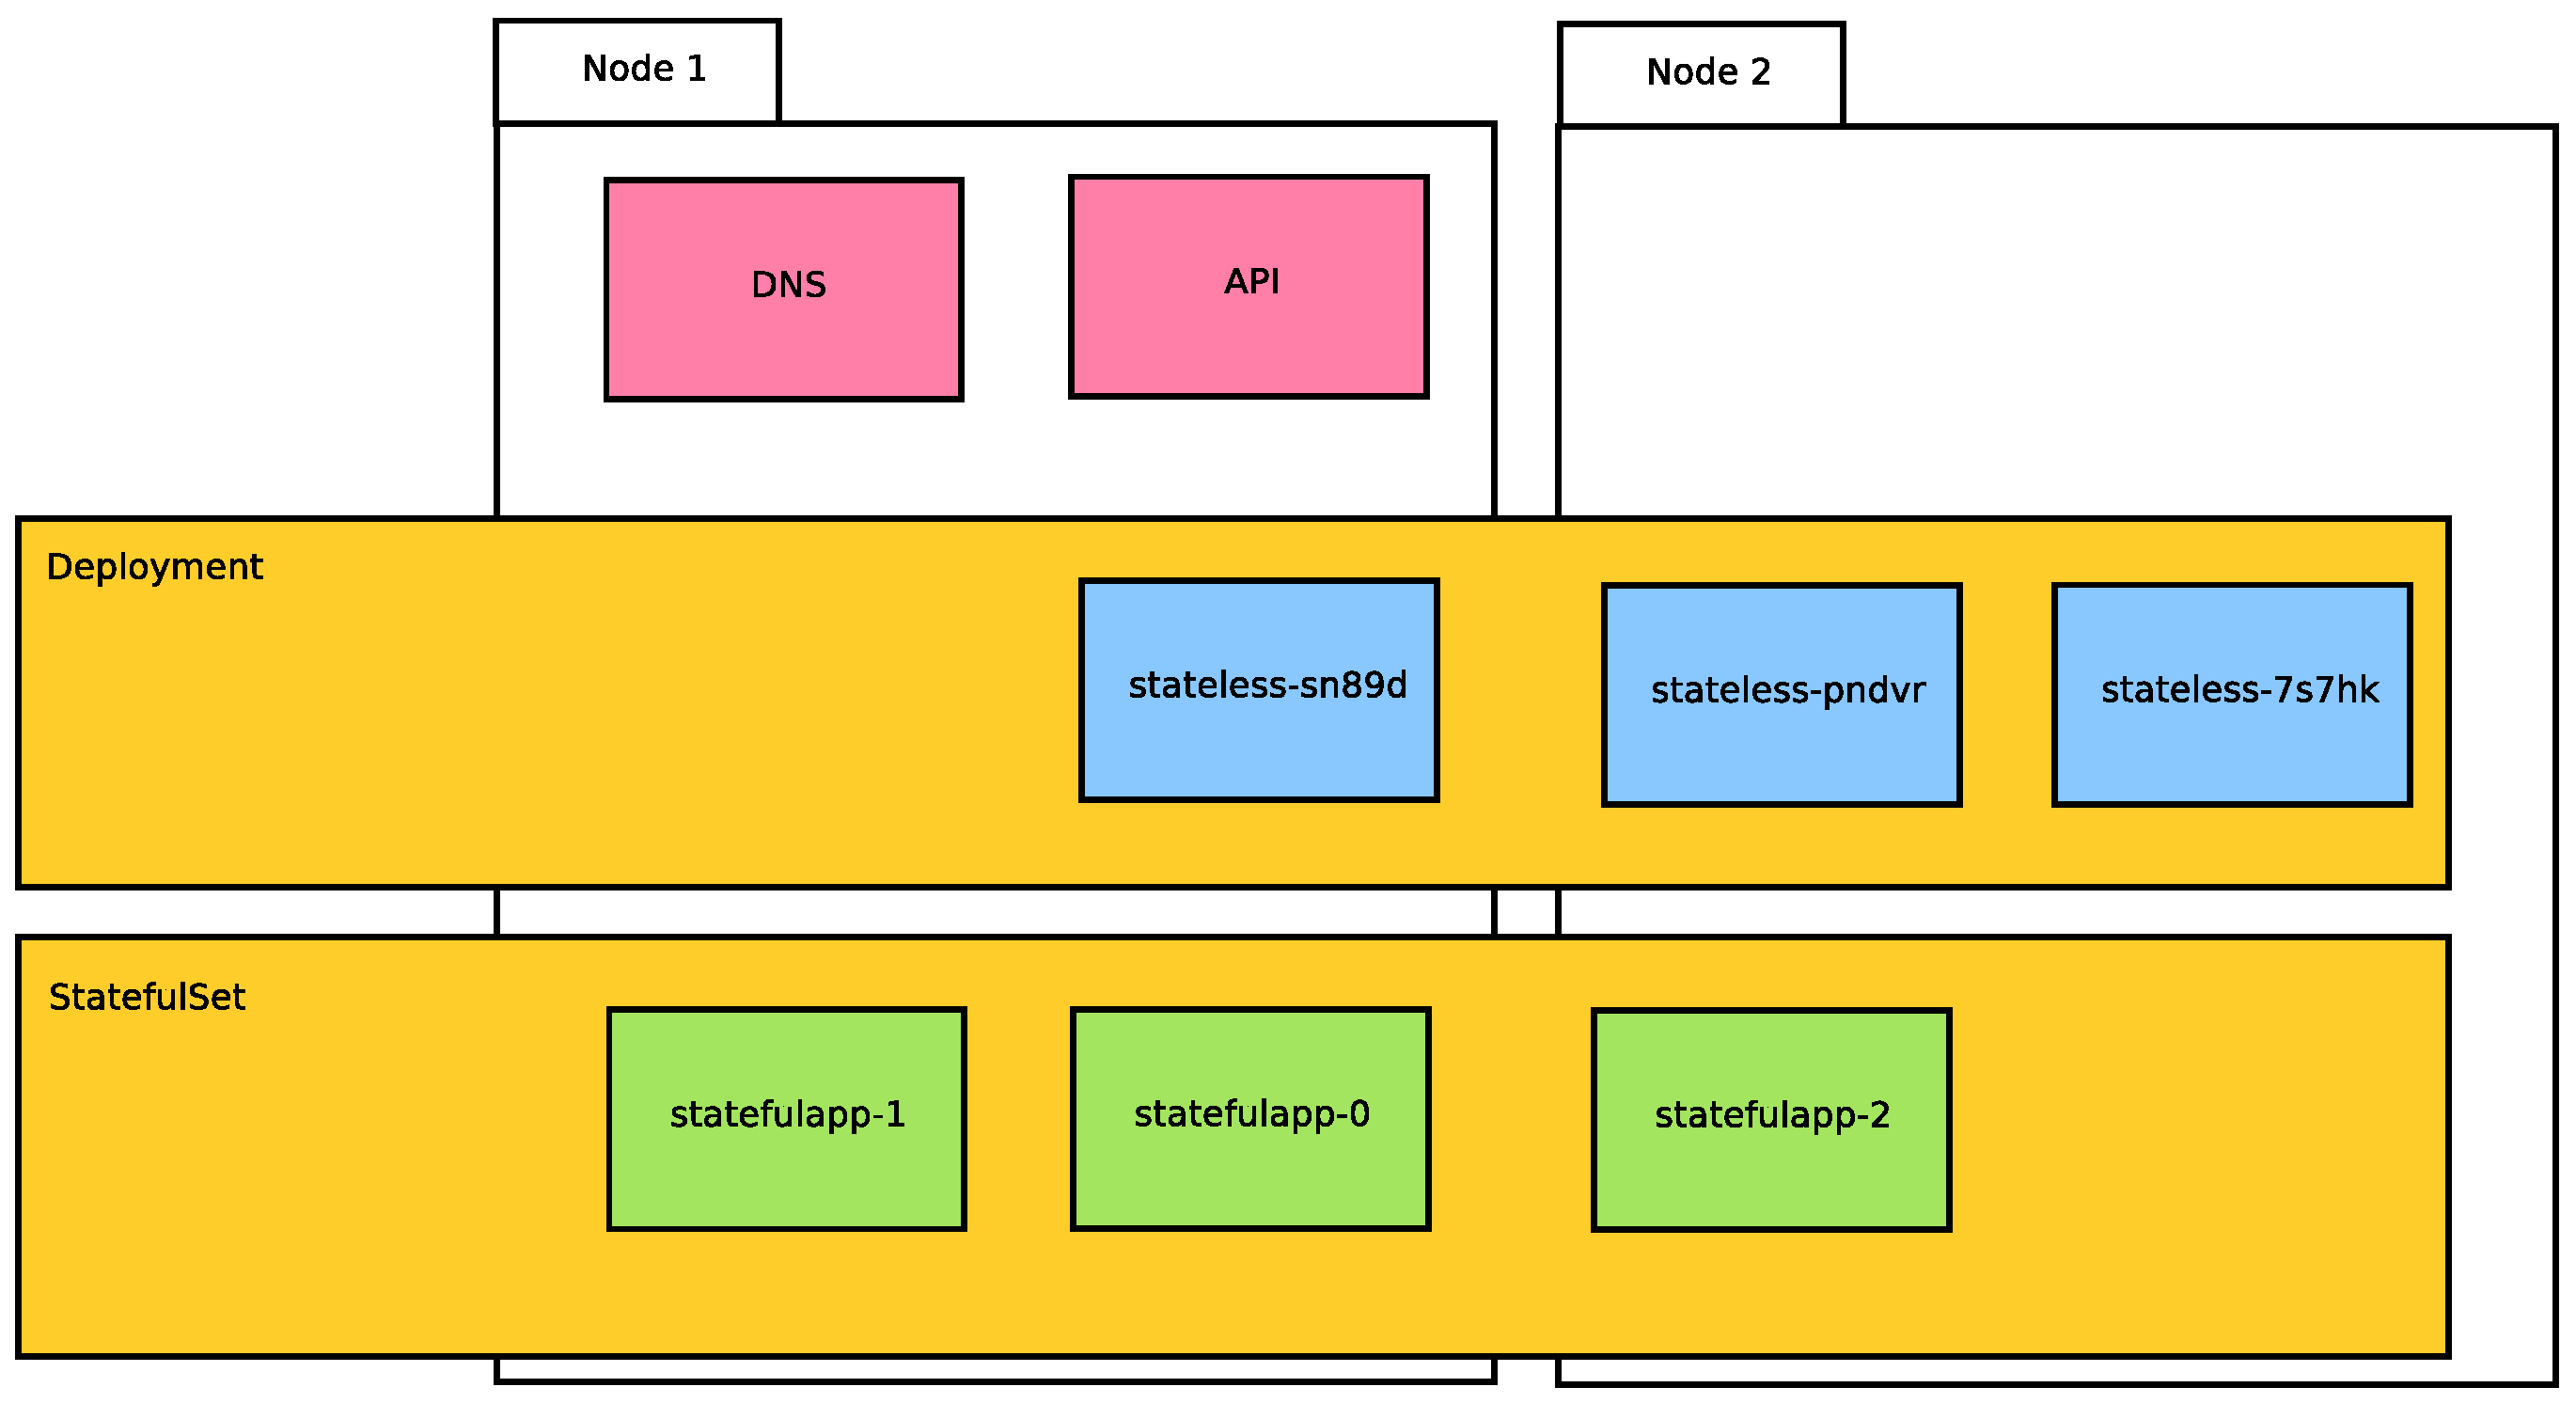
\includegraphics[width=\textwidth,height=0.85\textheight,keepaspectratio]{graphics/05-statefulSet.eps}
\end{frame}

\begin{frame}
    \frametitle{Persistent Storage}
    \begin{itemize}
        \item StatefulSet pod specifications allow you to create PersistentVolumeClaims.
        \item PVCs are used to request PersistentVolumes.
        \item PVs are beyond the scope of this presentation. Let's just say they are ``created on request".
    \end{itemize}
\end{frame}

\begin{frame}
    \frametitle{Persistent Storage}
    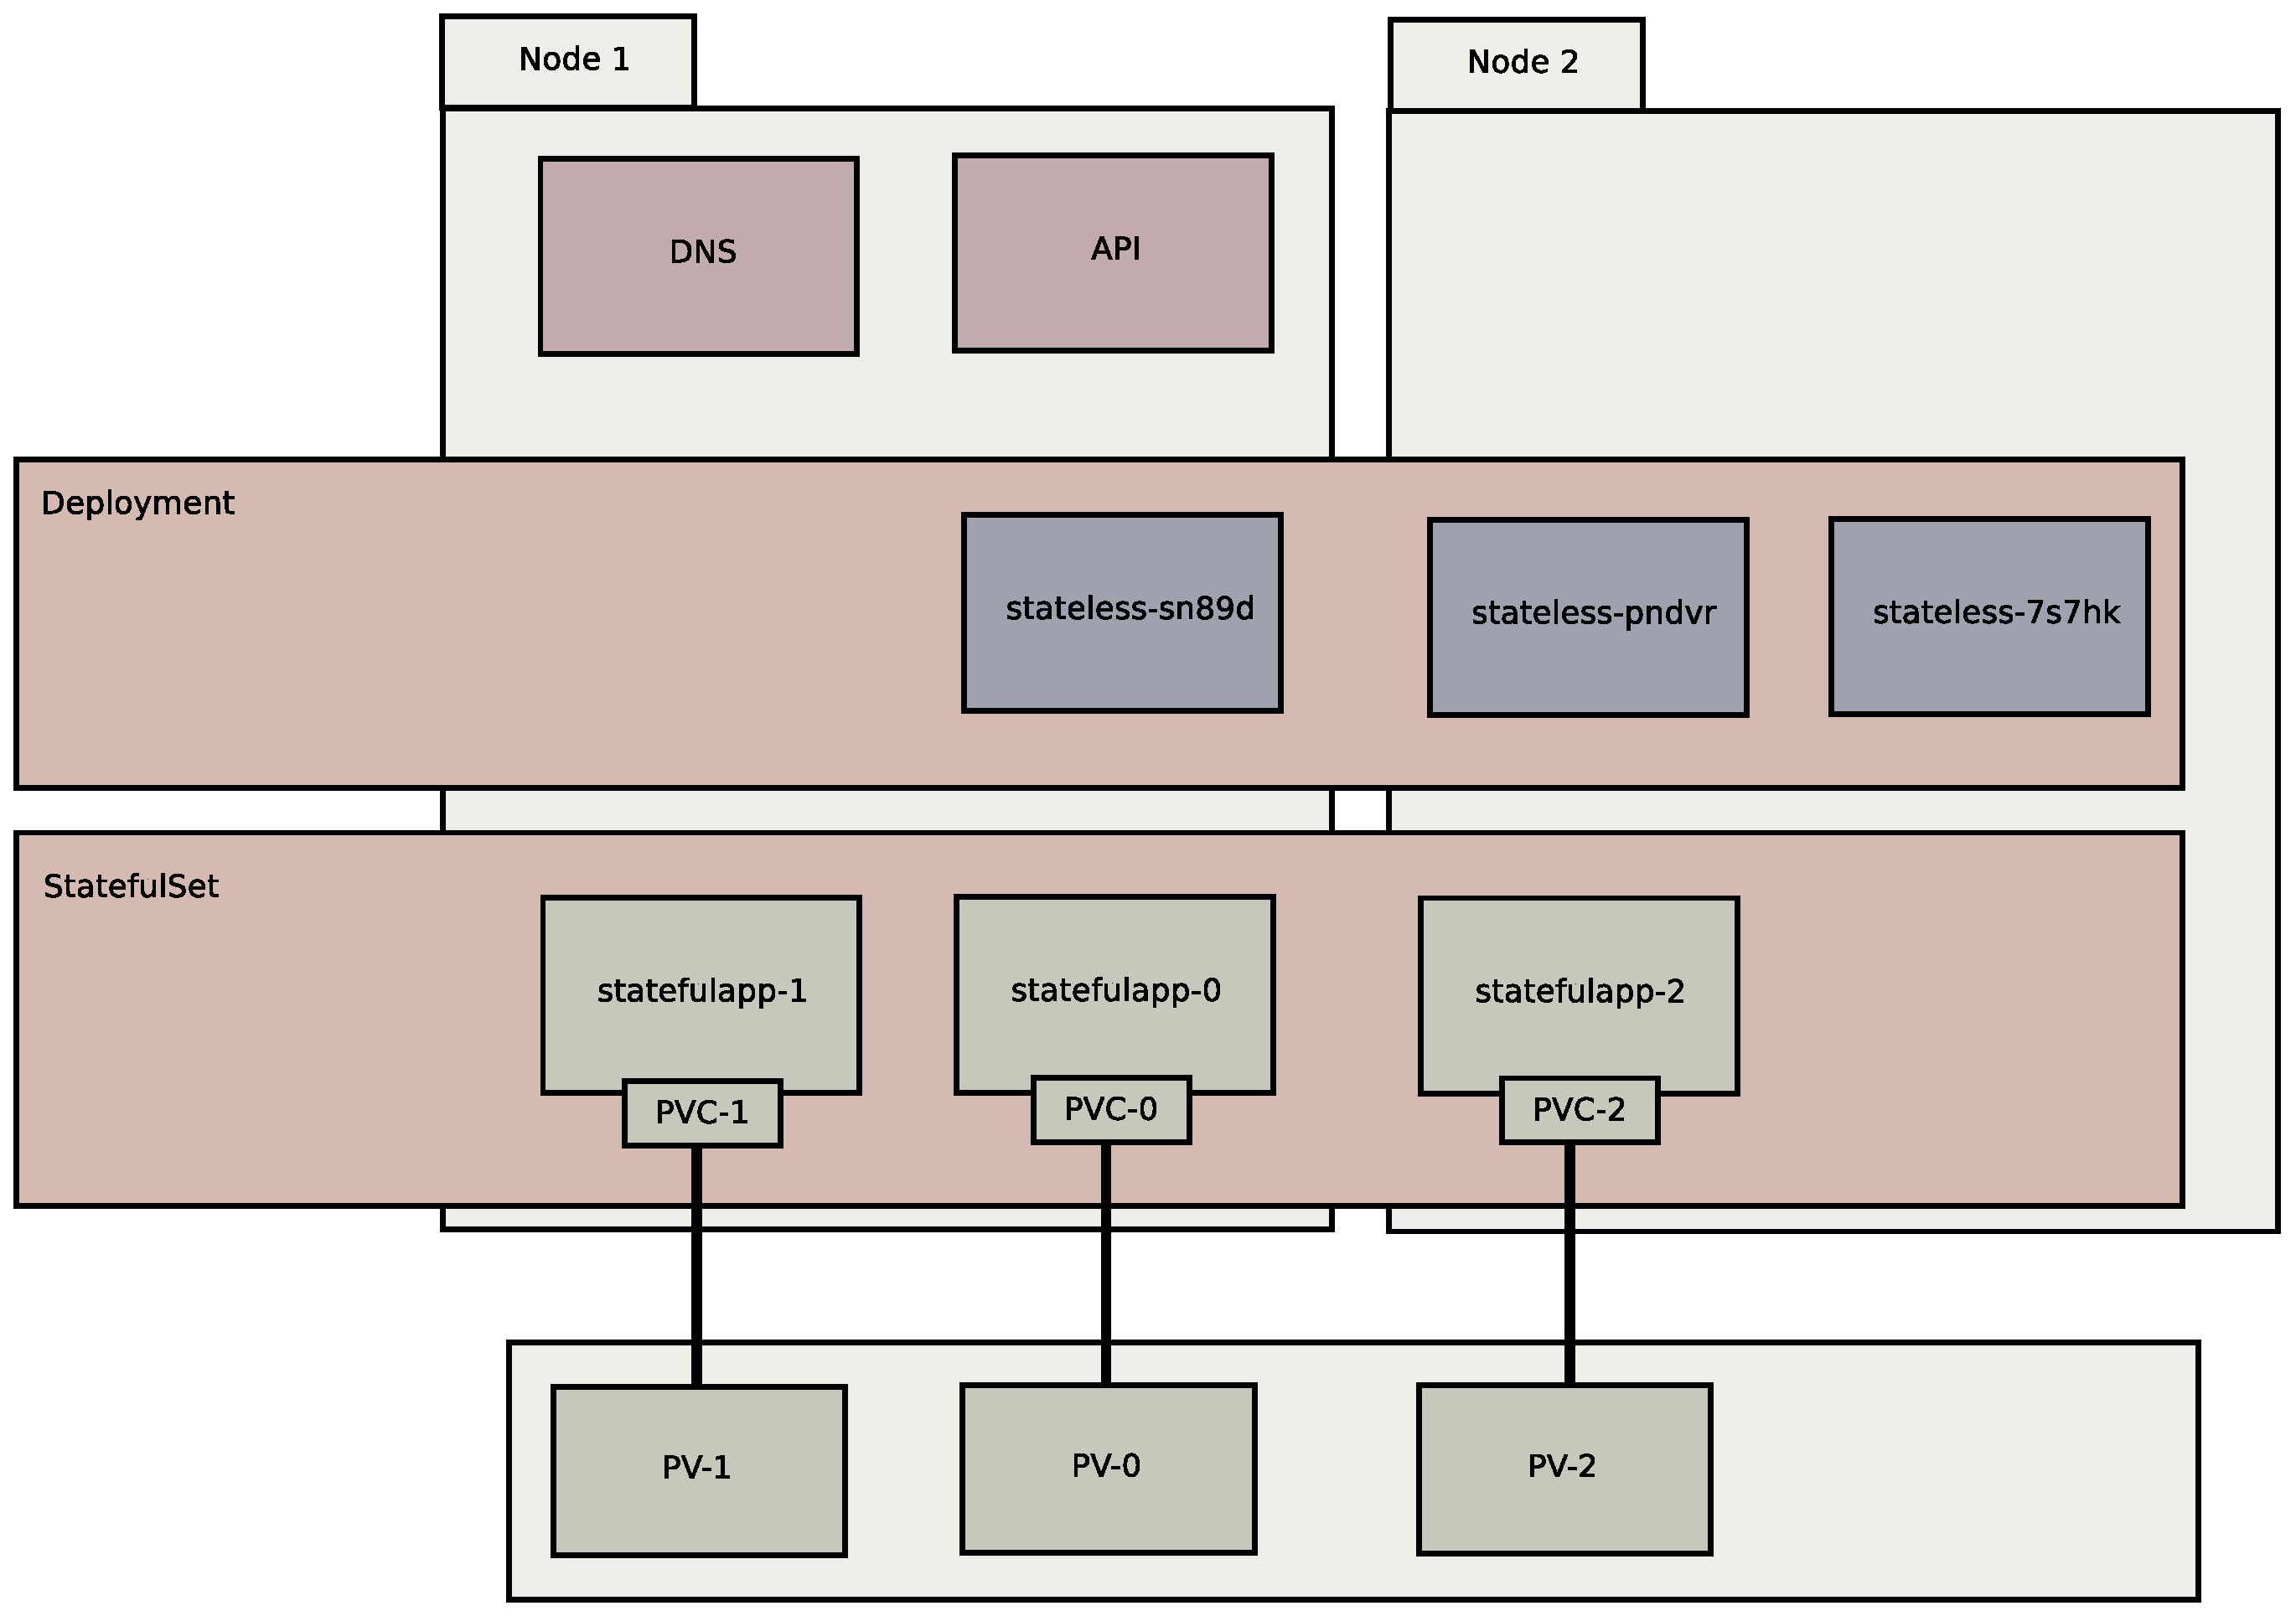
\includegraphics[width=\textwidth,height=0.85\textheight,keepaspectratio]{graphics/06-persistence.eps}
\end{frame}

\begin{frame}
    \frametitle{Headless Service}
    StatefulSets require a Headless Service
    \begin{itemize}
        \item A Headless Service is one without an IP address.
        \item It's used to manage DNS.
        \item It's what gives Pods in a StatefulSet a persistent network identity.
    \end{itemize}
\end{frame}

\begin{frame}
    \frametitle{Headless Service}
    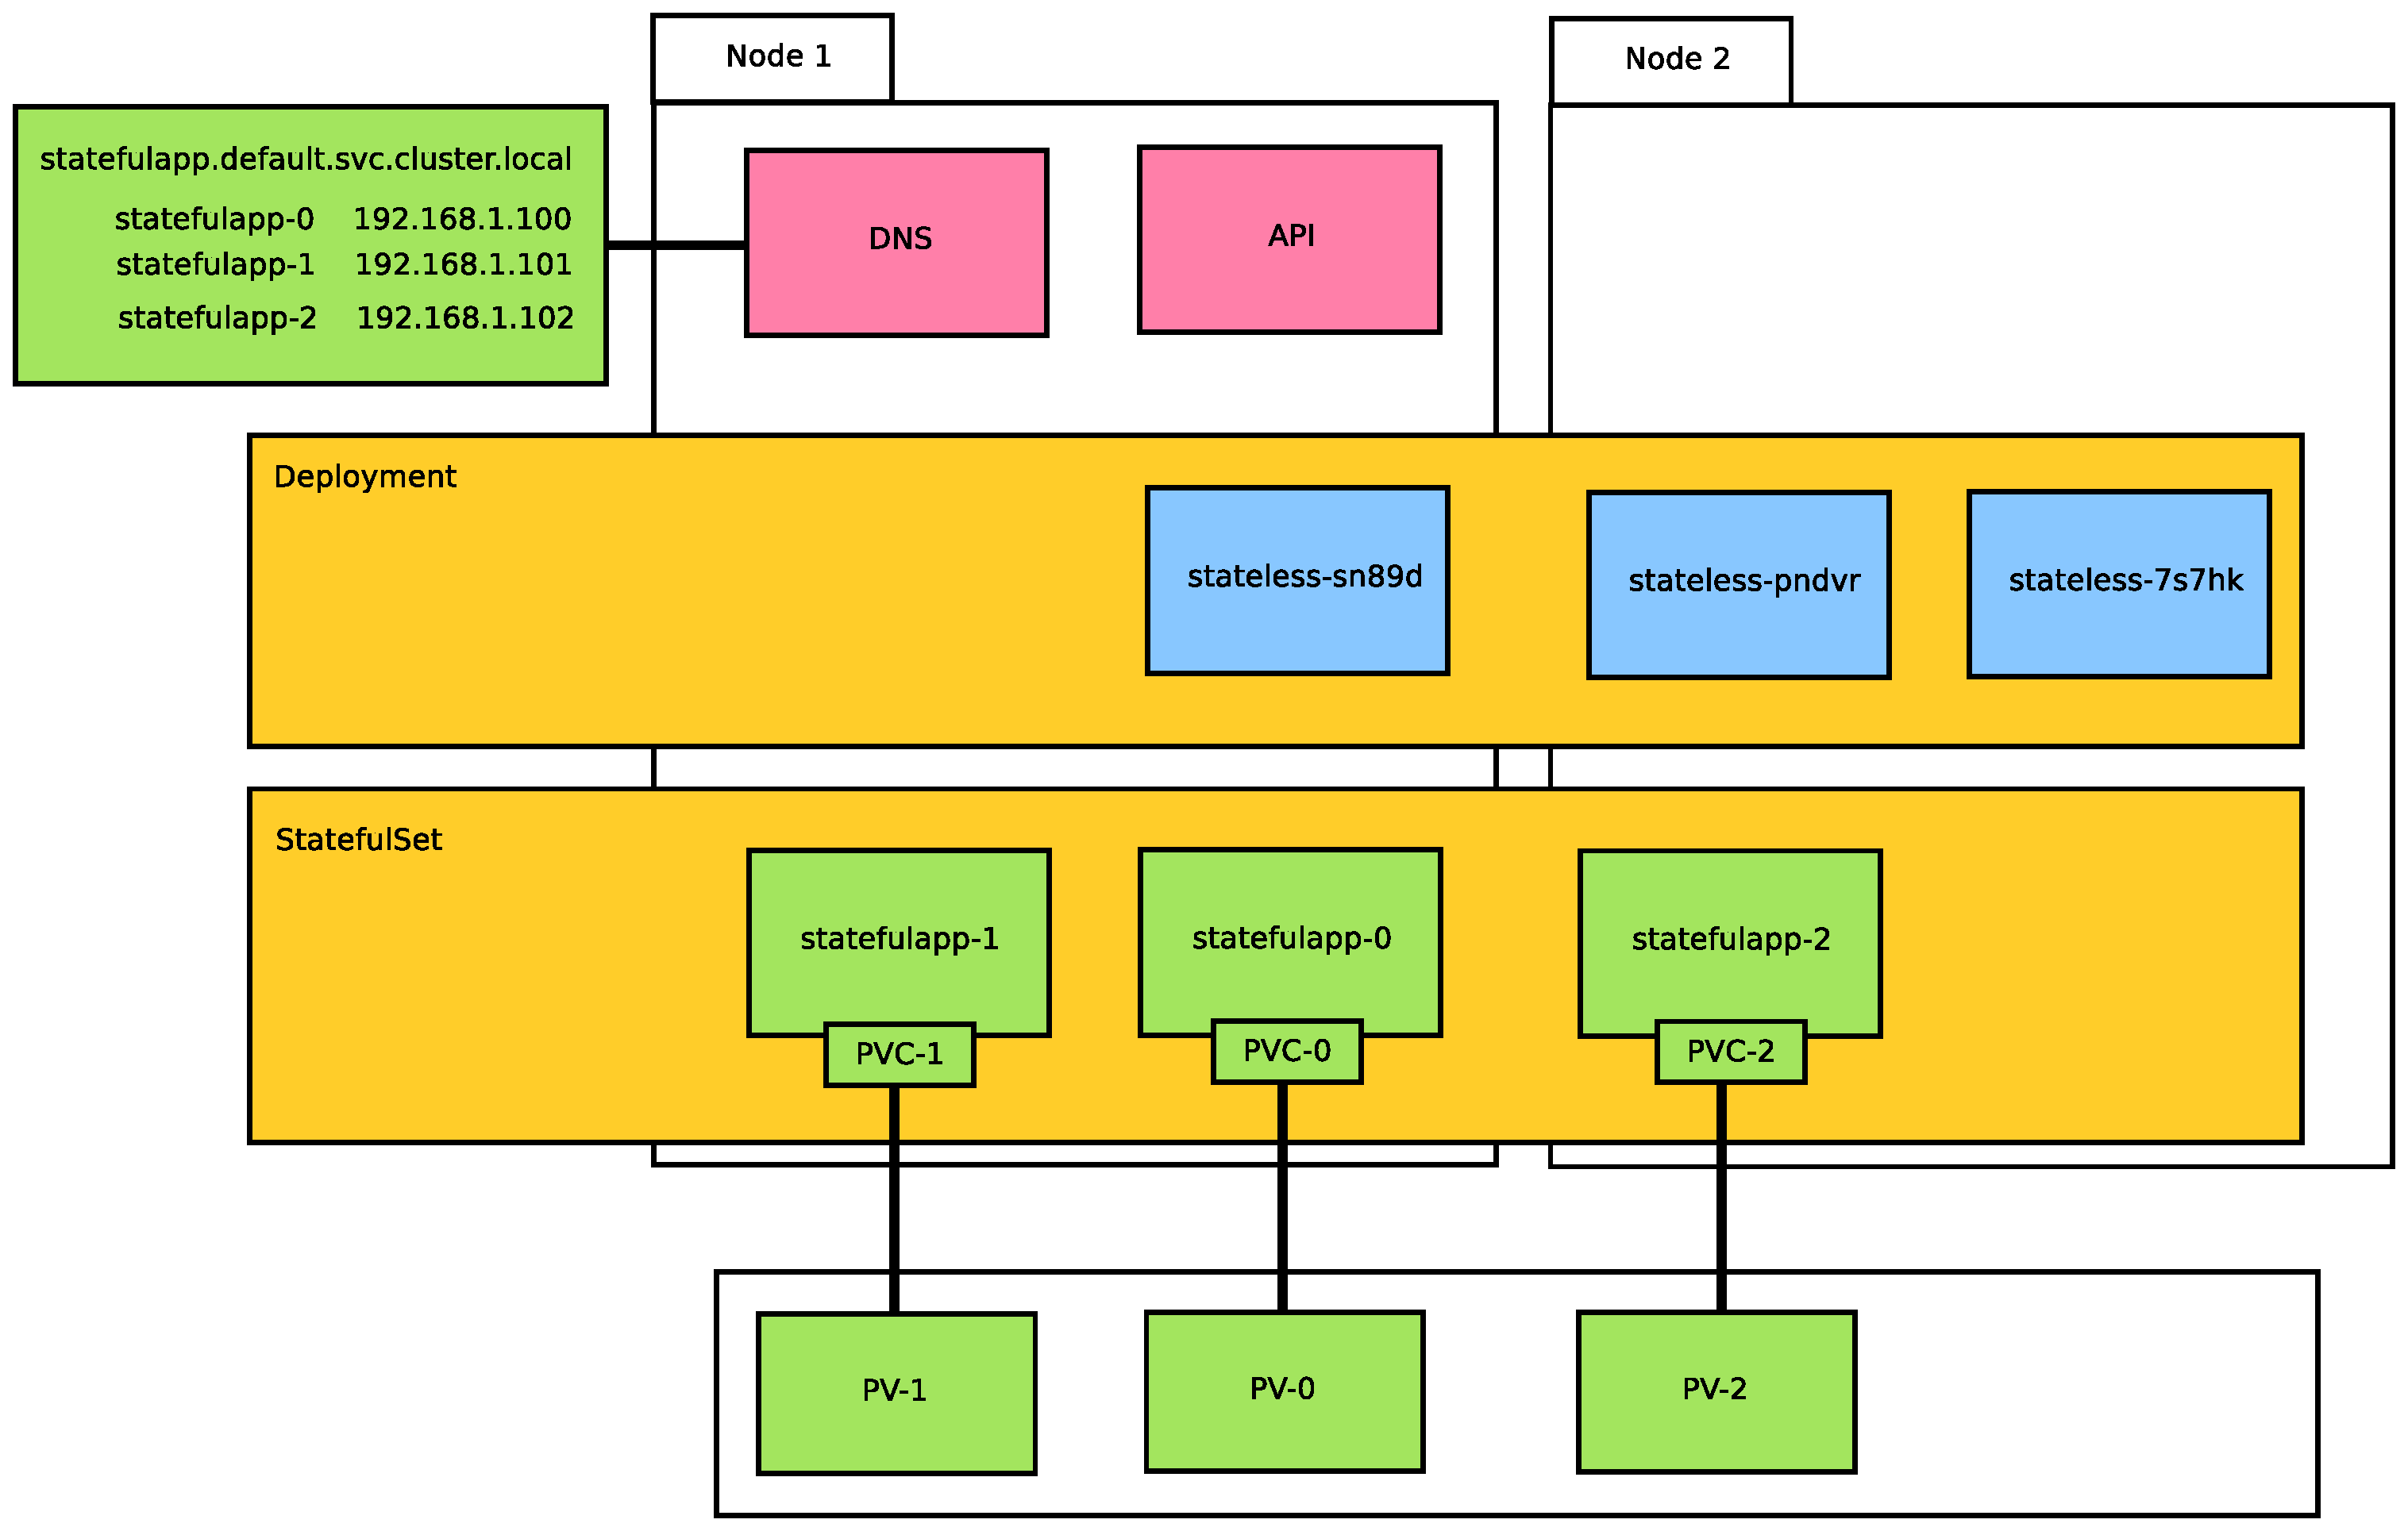
\includegraphics[width=\textwidth,height=0.85\textheight,keepaspectratio]{graphics/07-persistentIdentity.eps}
\end{frame}

\begin{frame}
    \frametitle{Load Balancers}
    \begin{itemize}
        \item Load Balancers have a "ClusterIP" and also an External IP.
        \item They balance requests sent to their IP address to all pods their "selector" targets.
    \end{itemize}
\end{frame}

\begin{frame}
    \frametitle{Load Balancing Services}
    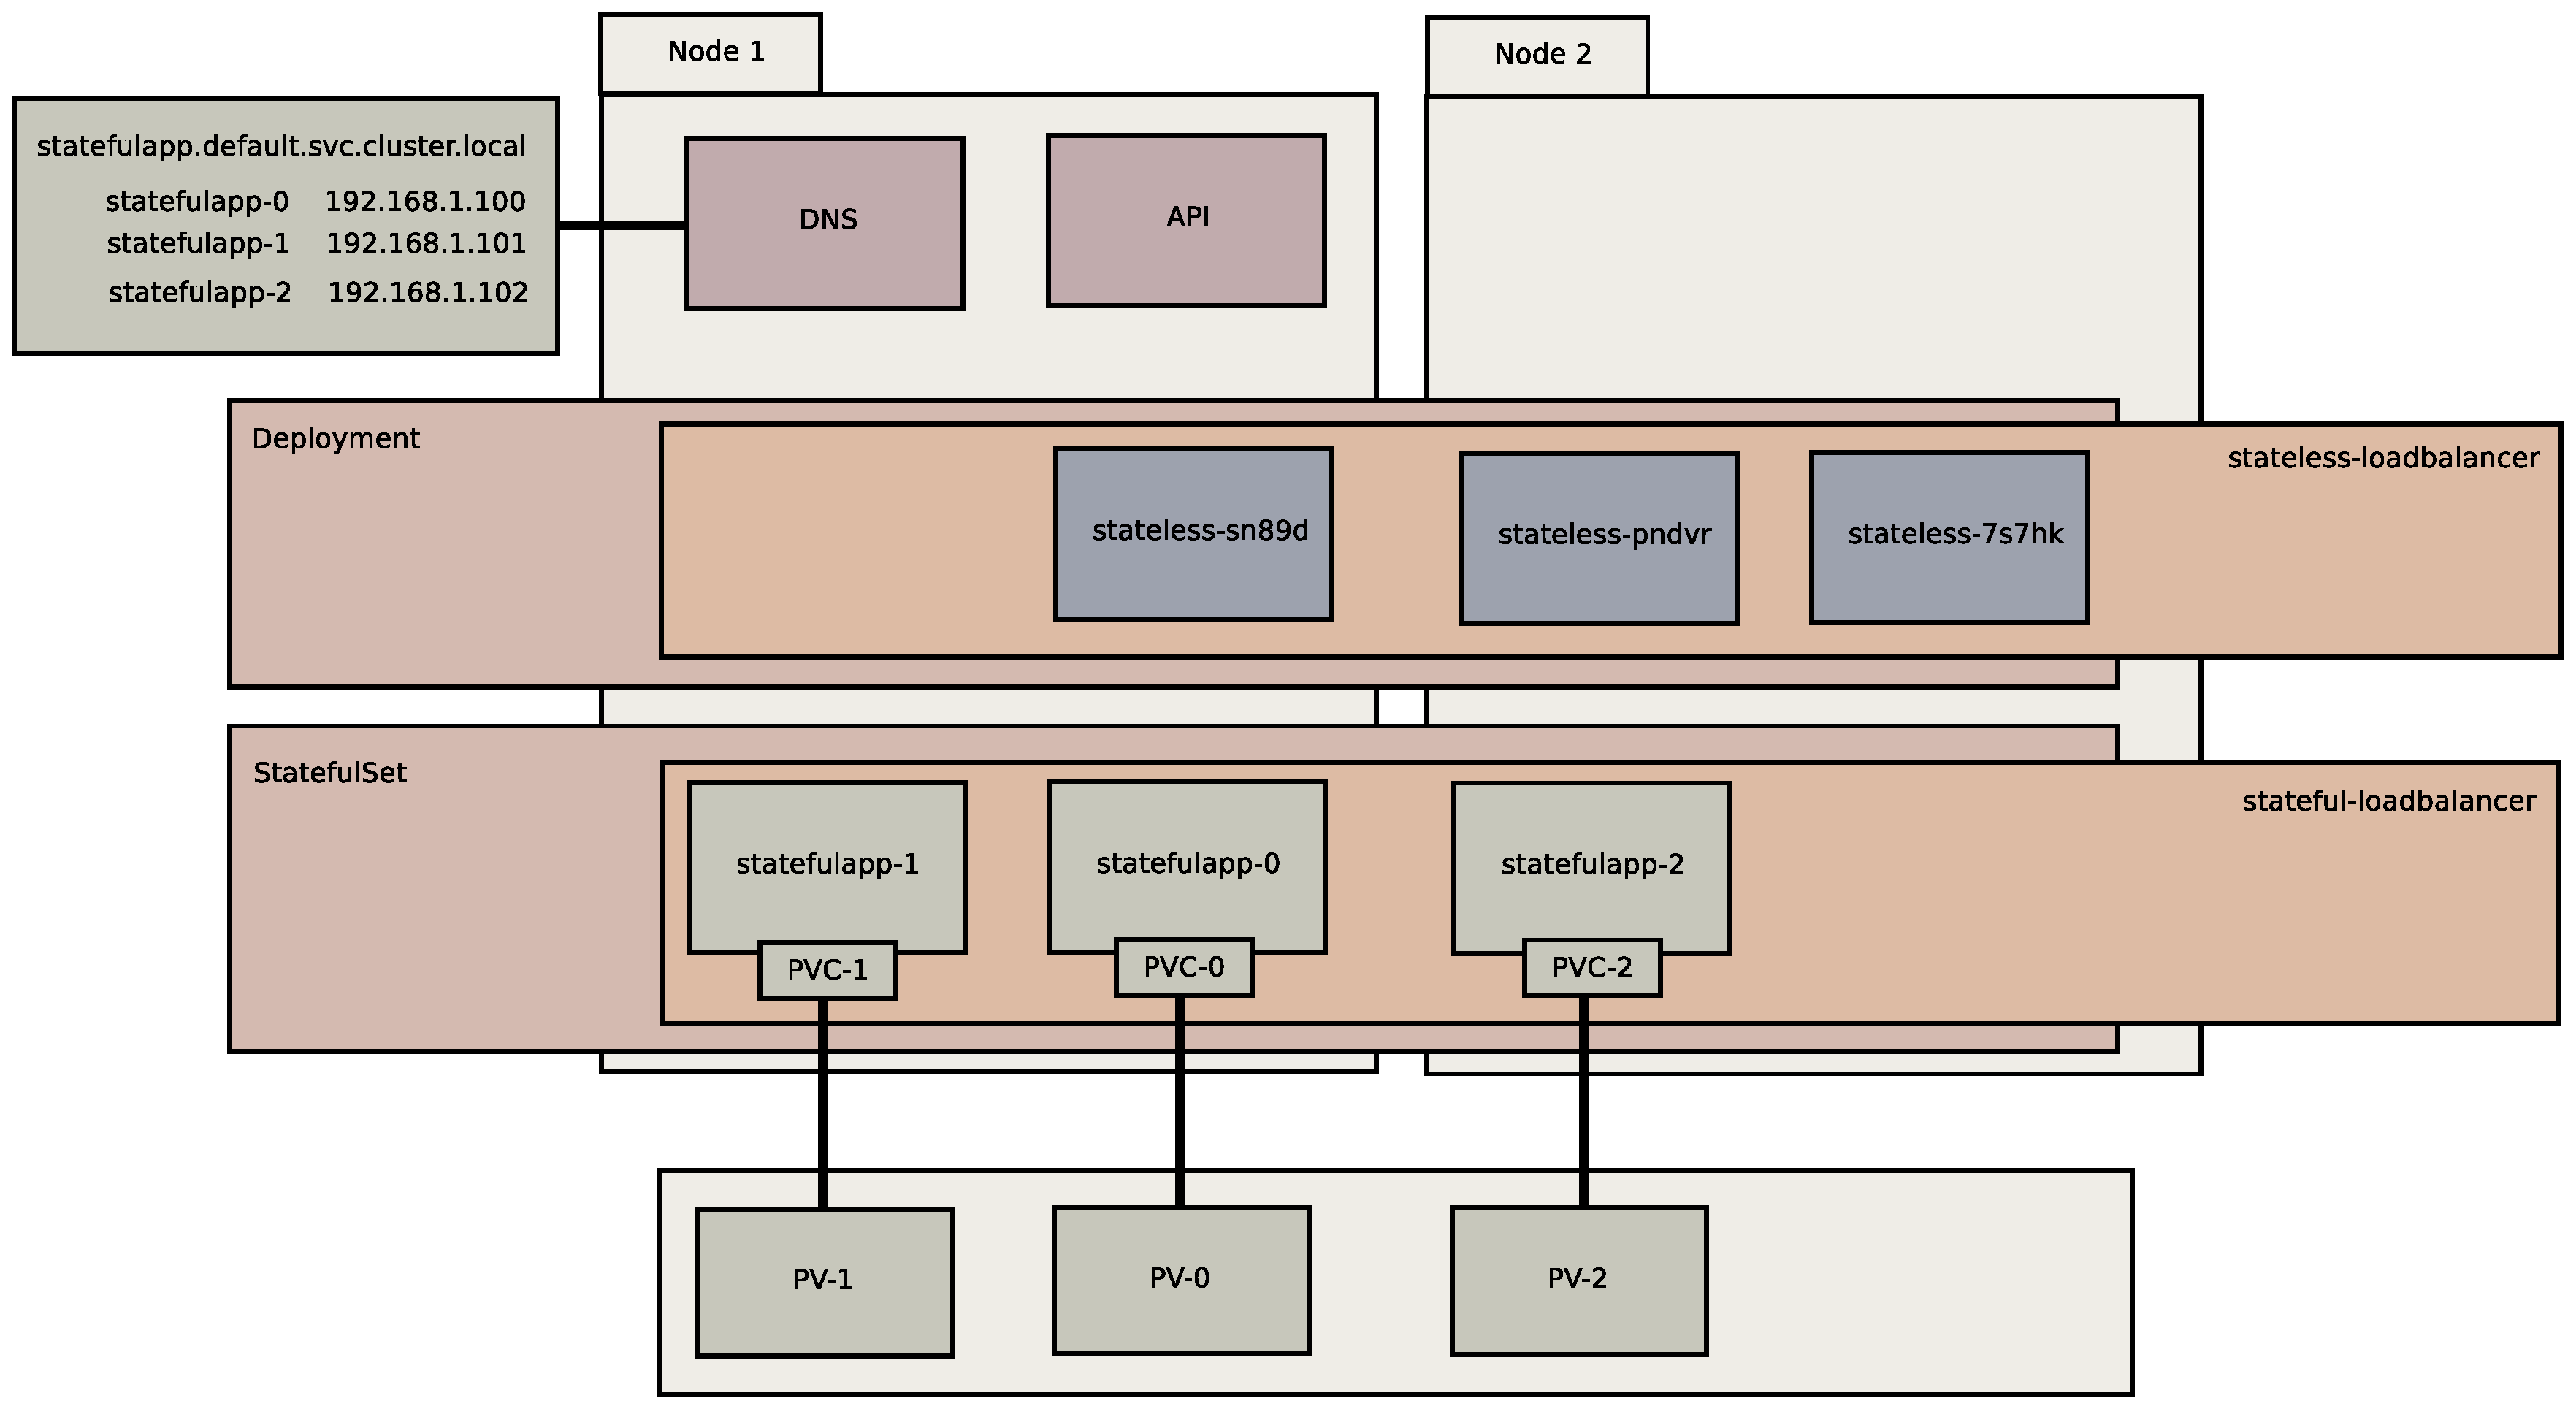
\includegraphics[width=\textwidth,height=0.85\textheight,keepaspectratio]{graphics/08-loadBalancer.eps}
\end{frame}

\begin{frame}
    \frametitle{Demo}
    \begin{center}
        \Huge So, let's see this in action!
    \end{center}
\end{frame}

\begin{frame}
    \frametitle{Overview}
    First, let's talk about the steps we're going to take:
    \begin{itemize}
        \item Start our Kubernetes environment (minikube).
        \item Configure our docker cli to talk to minikube's docker host.
        \item Build our two sample apps, package them as docker containers, and push the images.
        \item Run helm to deploy our applications.
        \item Proxy local ports to connect to our load balancing services.
    \end{itemize}
\end{frame}

\begin{frame}
    \frametitle{Demo}
    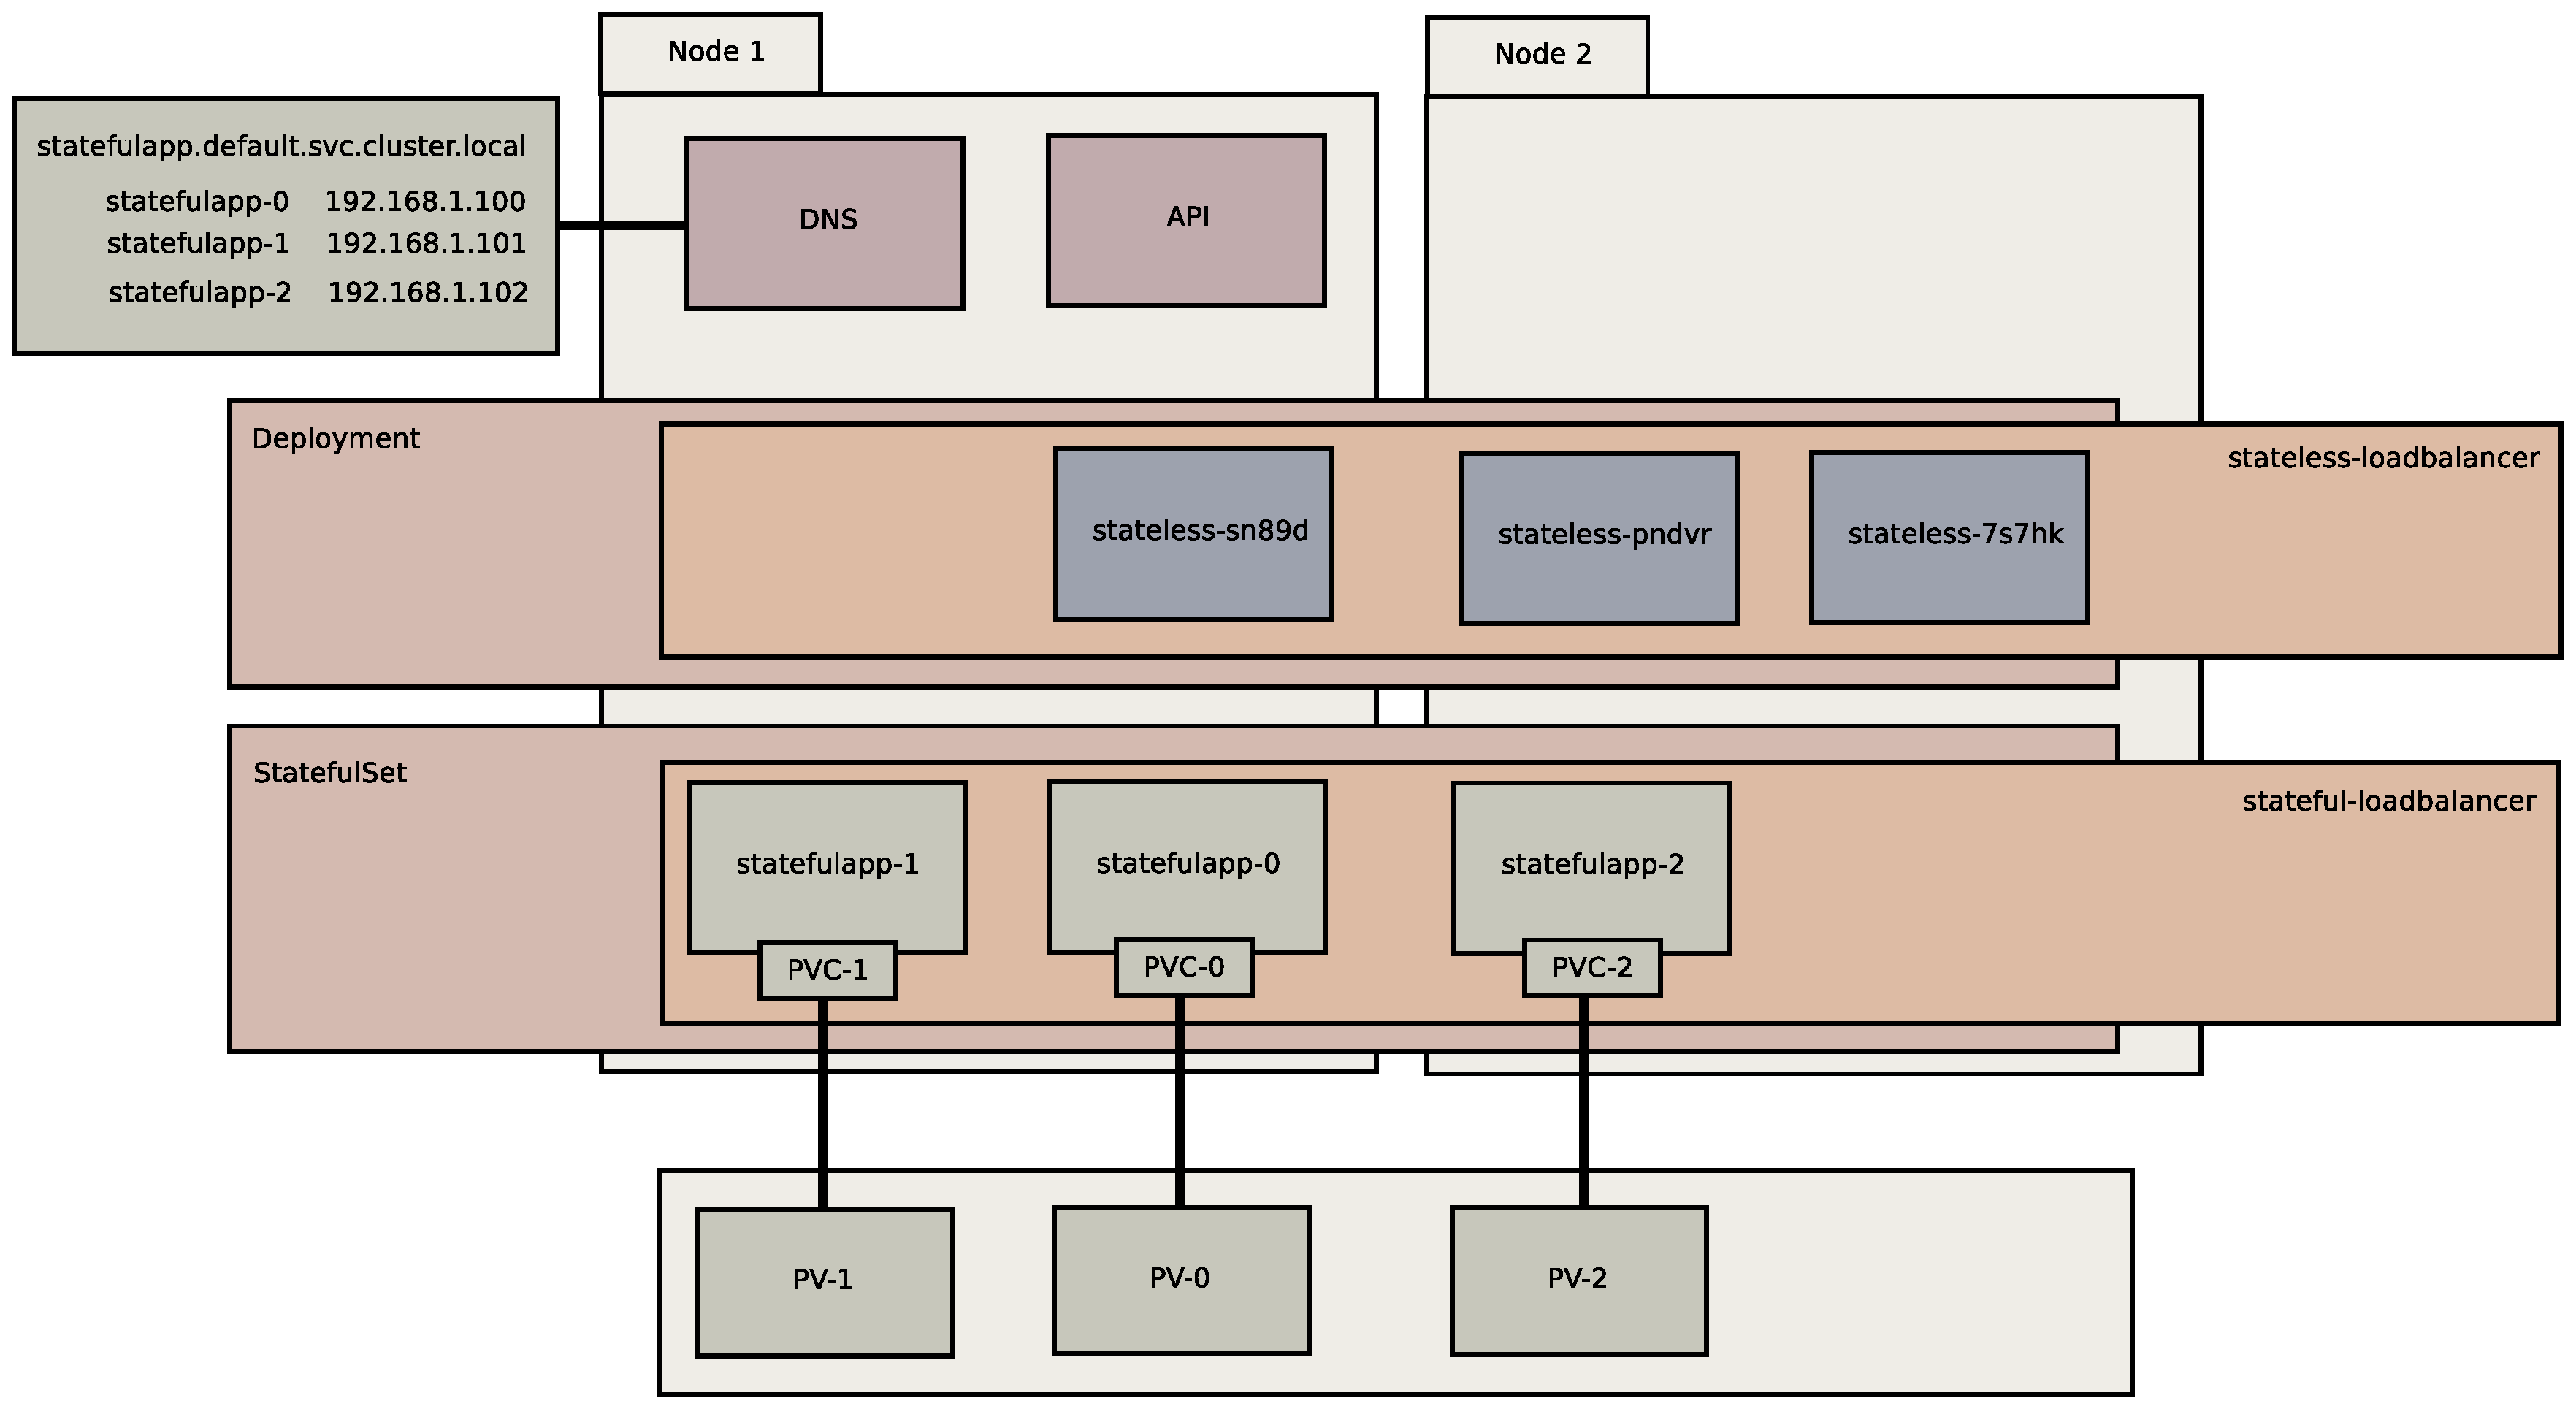
\includegraphics[width=\textwidth,height=0.85\textheight,keepaspectratio]{graphics/08-loadBalancer.eps}
\end{frame}

\begin{frame}
\frametitle{Other Resources}
Peripheral tools I used -- some of which warrant their own presentation
\begin{itemize}
    \item \LaTeX: \href{https://www.latex-project.org}{https://www.latex-project.org}
    \item Beamer: \href{https://ctan.org/pkg/beamer}{https://ctan.org/pkg/beamer}
    \item Kotlin: \href{https://kotlinlang.org}{https://kotlinlang.org}
    \item Spring Boot: \href{https://spring.io/projects/spring-boot}{https://spring.io/projects/spring-boot}
    \item Gradle: \href{https://gradle.org}{https://gradle.org}
    \item Dia: \href{http://dia-installer.de}{http://dia-installer.de}
\end{itemize}
\smallskip
Where I got my Subreddit data
\begin{itemize}
    \item Bulk Reddit data: \href{http://files.pushshift.io/reddit/subreddits}{http://files.pushshift.io/reddit/subreddits}
\end{itemize}
Finally, \textbf{\textit{this}} demo
\begin{itemize}
    \item \href{https://github.com/emacdona/k8sdemo}{https://github.com/emacdona/k8sdemo}
\end{itemize}
\end{frame}

\begin{frame}
    \begin{center}
        \Huge Questions?
    \end{center}
\end{frame}

\end{document}
